\qrchapter{https://forgottenpillar.com/rsc/en-fp-chapter23}{The great apostasy is soon to be realized} \label{chap:apostasy}

In 1903, when the Living Temple was published and instigated the controversy over the \emcap{personality of God}, Sister White was faithfully obeying the command of the Great Commander. She was called by the words “\textit{Meet it!}” She faced this controversy by writing numerous letters to many people in the field. In these letters, we trace the prophetic insight of the future of the Seventh-day Adventist Church.

One example is the correspondence between Sister White and her son William White. On November 26, 1905, there was a great Health Conference in College View Nebraska, where many medical missionary workers met together. William White was there and he had a short, 30-minute public talk. Afterwards, he wrote a letter to his mother regarding his impressions from the conference. Here is part of that letter: 

\others{College View, Ne. – Tuesday, November 28, 1905; Author: William C. White} \\
\others{Nov. 28, 1905.} \\
\others{Mrs. E. G. White, Sanitarium, Cala.}

\othersnogap{...Sabbath morning I had opportunity to speak about thirty minutes. In my remarks I refered to the history of the Christian church. They began with pure principles, but through the attacks of Satan they became backslidden and departed from those principles. \textbf{I pointed out that the only hope for the S. D. A. church was to \underline{adhear to first principles}}. \textbf{I then referred to the order in which the enemy is attacking our work. His first effort was to destroy union and establish separation. His next work was to weaken our reverence for the Sabbath, then to weaken our faith in the Sanctuary service, then \underline{to break our confidence in the Spirit of Prophecy}, then to \underline{confuse our conception regarding a personal God}}.}[Letter from W. C. White to E. G. White, November 28, 1905.][http://ellenwhite.org/content/correspondence/incoming/43292pdf]

\begin{figure}
    \centering
    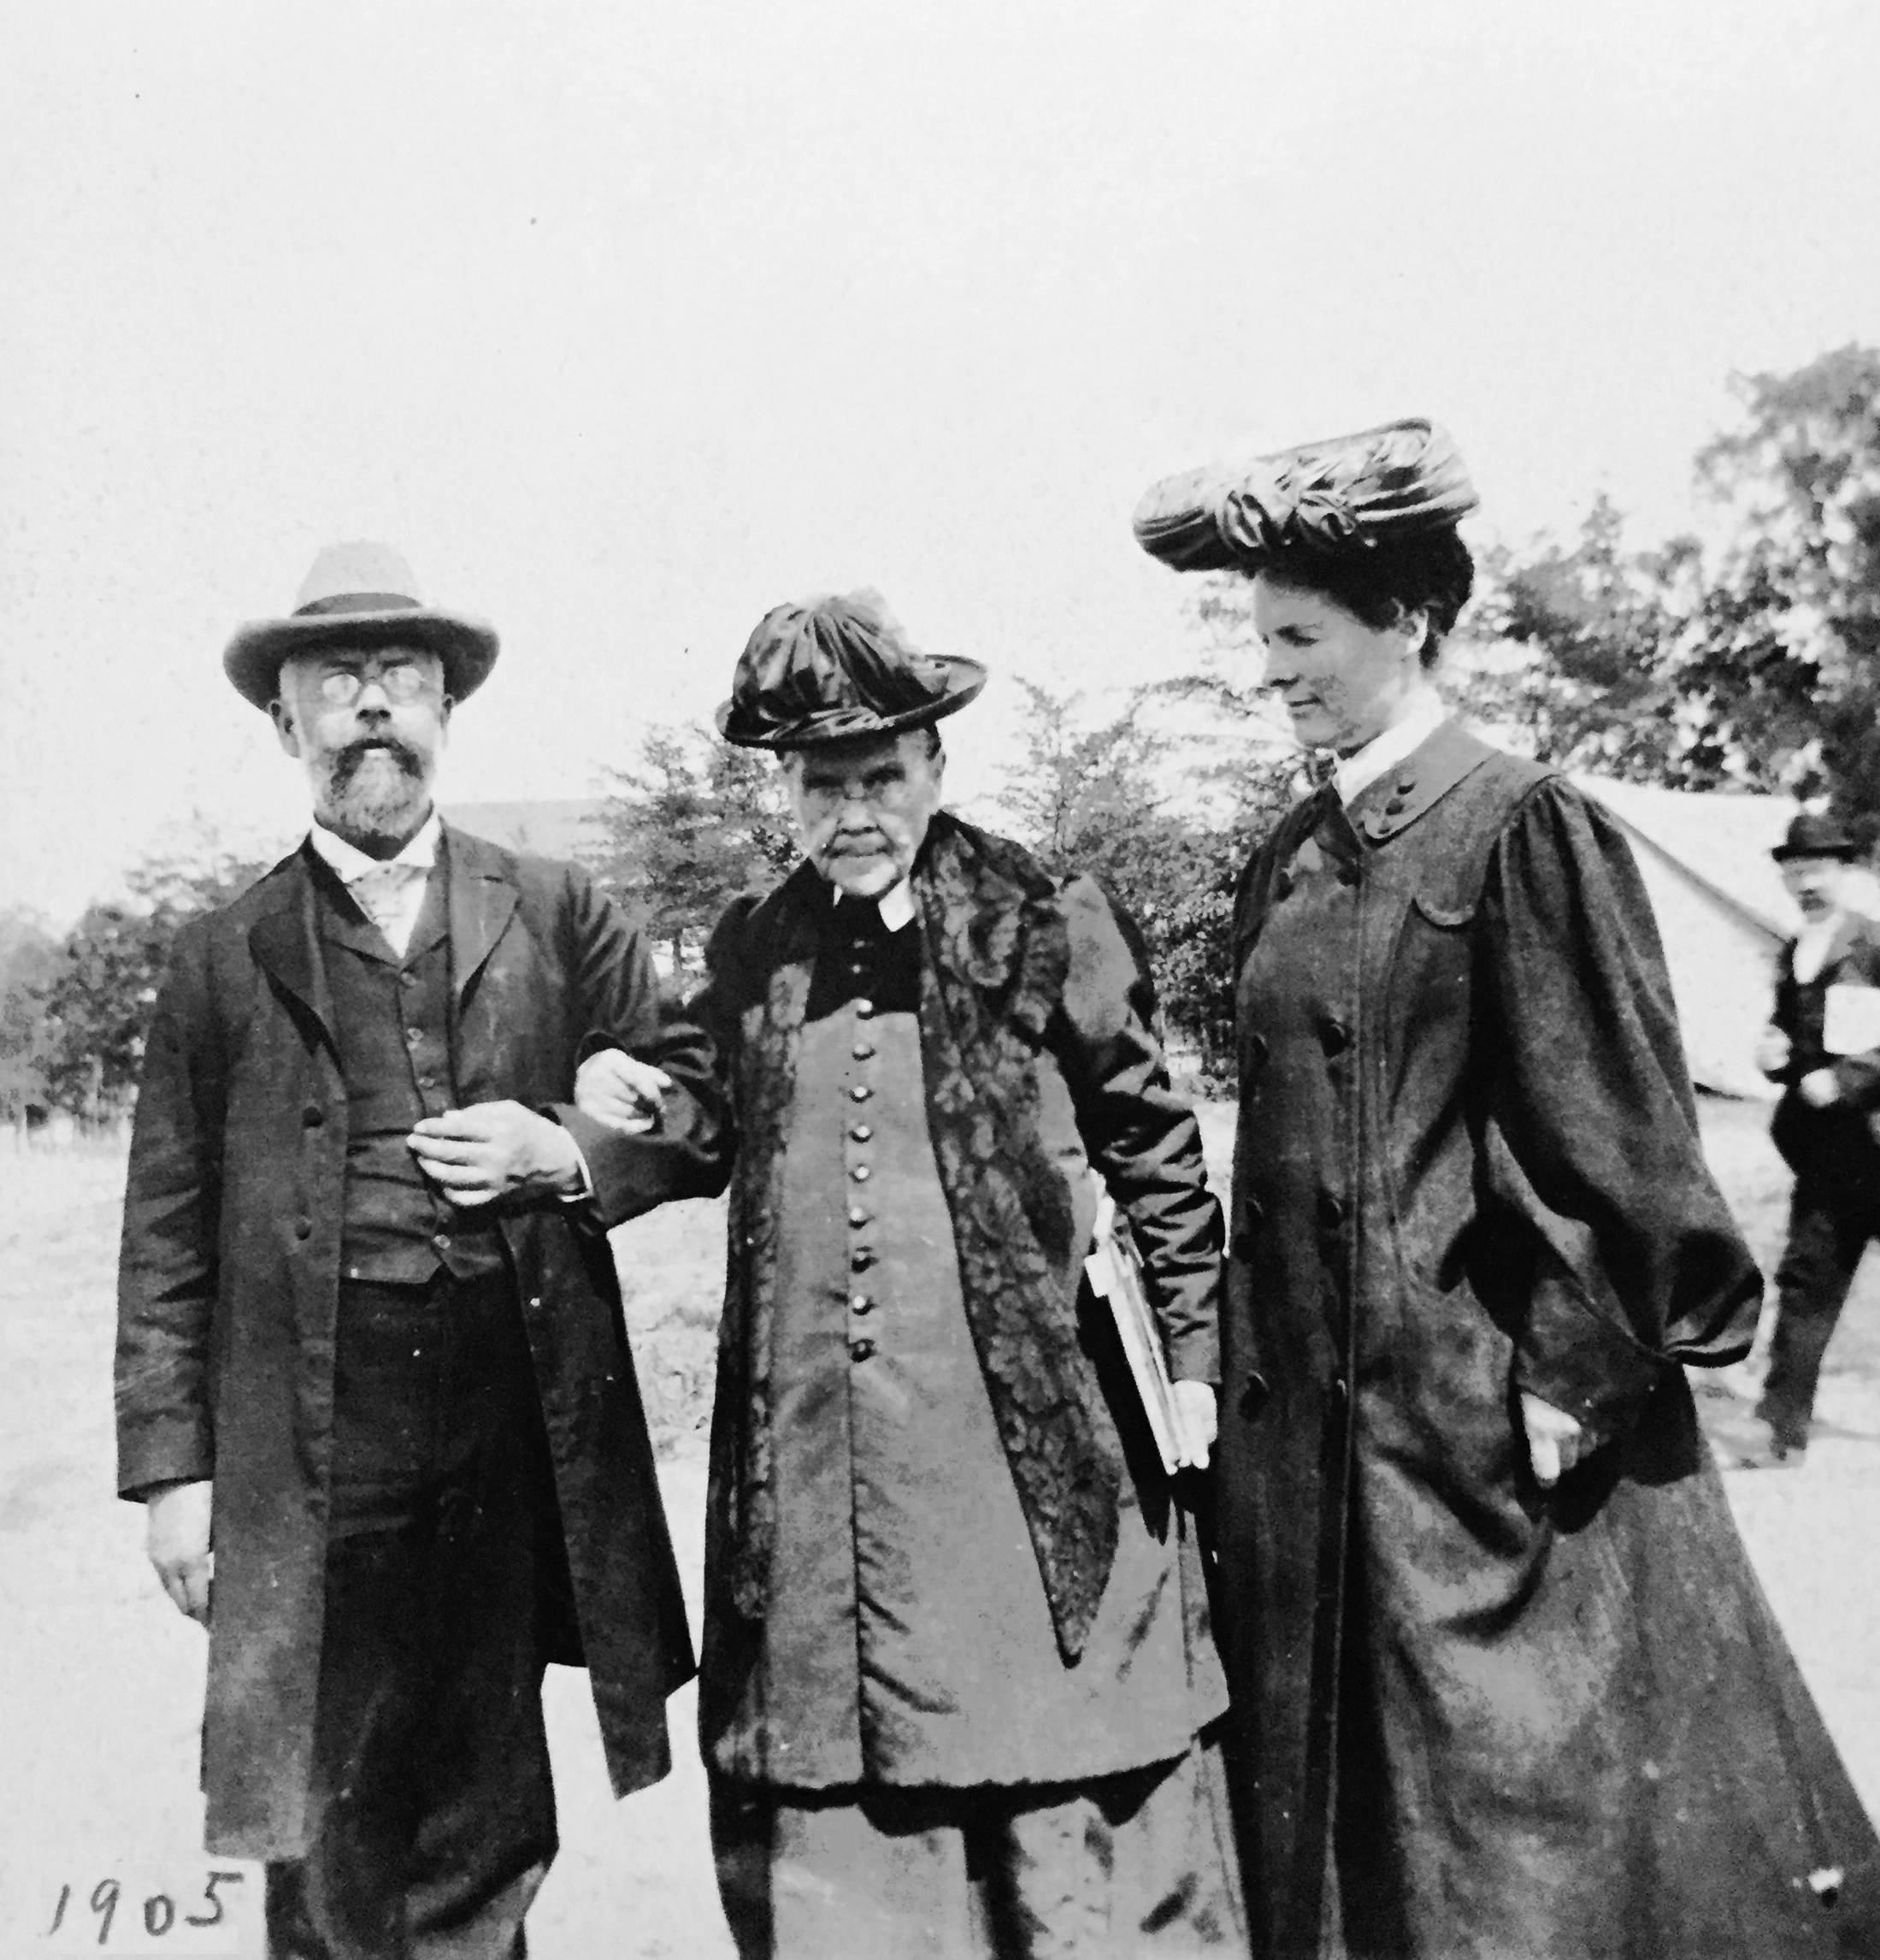
\includegraphics[width=1\linewidth]{images/william-ellen-white-1905.jpg}
    \caption*{William C. White and Ellen G. White, 1905}
    \label{fig:w-e-white}
\end{figure}

According to William White, our only hope as Seventh-day Adventists is to adhere to first principles. These principles, as we know, are the \emcap{Fundamental Principles}. Then, he referred to the order in which the enemy is attacking our work. The attack begins with our disunity, then aims to weaken our reverence for the Sabbath and the Sanctuary service, targets our confidence in the Spirit of Prophecy, and finally focuses on confusing our conceptions regarding personal God.

Sister White’s response to William White is of a startling nature. She hints to us that the great apostasy is soon to be realized, and that our hope is to adhere to the first principles of our faith—the \emcap{Fundamental Principles}.

\egw{Elmshaven, St. Helena, California} \\
\egw{December 4, 1905} \\
\egw{W. C. White} \\
\egw{My dear son - }

\egw{...}

\egw{“\textbf{One thing it is certain is soon to be realized—\underline{the great apostasy}, which is developing and increasing and waxing stronger and \underline{will continue} to do so until the Lord shall descend from heaven with a shout. \underline{We are to hold fast the first principles of our denominated faith} and go forward from strength to increased faith. \underline{Ever} we are to keep the faith that has been substantiated by the Holy Spirit of God \underline{from the earlier events of our experience until the present time}.} We need now larger breadth and deeper, more earnest, unwavering faith in the leadings of the Holy Spirit. \textbf{If we needed the manifest proof of the Holy Spirit’s power to confirm truth \underline{in the beginning}, after the passing of the time, \underline{we need today all the evidence in the confirmation of the truth}, when souls are departing from the faith and giving heed to seducing spirits and doctrines of devils.} There must not be any languishing of soul now. If ever there was a period of time when we needed the Holy Spirit’s power in our discourses, in our prayers, in every action proposed, it is now. \textbf{We are not to stop at the first experience, but while we bear \underline{the same message} to the people, \underline{this message is to be strengthened and enlarged}}. \textbf{We are to see and realize the importance of the message made certain by its divine origin}. We are to follow on to know the Lord, that we may know that His going forth is prepared as the morning. Our souls need the quickening from the Source of all power. \textbf{We may be strengthened and confirmed in the past experience \underline{that holds us to the essential points of truth which have made us what we are—Seventh-day Adventists}.}“}[Lt326-1905.2; 1905][https://egwwritings.org/read?panels=p7678.8]

\egwnogap{\textbf{The past fifty years have not dimmed one jot or principle of our faith as we received the great and wonderful evidences that were made certain to us in 1844, after the passing of the time.} The languishing souls are to be confirmed and quickened according to His Word. And many of the ministers of the gospel and the Lord’s physicians will have their languishing souls quickened according to the Word. \textbf{\underline{Not a word is changed or denied}.} \textbf{That which the Holy Spirit testified to as truth after the passing of the time, in our great disappointment, is \underline{the solid foundation of truth}. Pillars of truth were revealed, and we accepted \underline{the foundation principles} that have made us what we are—Seventh-day Adventists, keeping the commandments of God and having the faith of Jesus.}}[Lt326-1905.3; 1905][https://egwwritings.org/read?panels=p7678.9]

This letter is startling because it is an answer to the order of how the enemy is attacking our work. Sister White is well aware of these attacks and she presented the problem in its correct light, also showing us what we shall do to prevent Satan's attacks on us. The enemy wants to \others{confuse our conception regarding a personal God}. This is the very point of great apostasy that \egwinline{is soon to be realized}, and has been \egwinline{developing and increasing and waxing stronger and will continue to do so until the Lord shall descend from heaven with a shout}. This is the apostasy we are experiencing today. What is our hope against this deception and great apostasy? \egwinline{\textbf{\underline{We are to hold fast the first principles of our denominated faith} and go forward from strength to increased faith. \underline{Ever} we are to keep the faith that has been substantiated by the Holy Spirit of God from the earlier events of our experience until the present time.}} \egwinline{...\textbf{\underline{this message is to be strengthened and enlarged}}...} \egwinline{...\textbf{\underline{we need today all the evidence in the confirmation of the truth}}...} \egwinline{\textbf{We may be strengthened and confirmed in the past experience that holds us to the essential points of truth which have made us what we are—Seventh-day Adventists}}. These essential points of truth, which have made us Seventh-day Adventists, are the \emcap{Fundamental Principles}, born in the beginning of our work. In 1905, she wrote, \egwinline{\textbf{The past fifty years have not dimmed one jot or principle of our faith as we received the great and wonderful evidences that were made certain to us in 1844, after the passing of the time.}} \egwinline{\textbf{Not a word is changed or denied.} \textbf{That which the Holy Spirit testified to as truth after the passing of the time, in our great disappointment, is \underline{the solid foundation of truth}. Pillars of truth were revealed, and we accepted \underline{the foundation principles} that have made us what we are—Seventh-day Adventists, keeping the commandments of God and having the faith of Jesus.}}

God calls us to be steadfast in the \emcap{Fundamental Principles}, especially over the \others{conception regarding a personal God}. This is the first point of the \emcap{Fundamental Principles}.

Sister White foretold that a great apostasy is developing in our church regarding the understanding of the \emcap{personality of God}. The true understanding of the \emcap{personality of God} is presented in the \emcap{Fundamental Principles}. She clearly warned us of Satan’s attack on these principles. She calls us to \egw{\textbf{hold fast the first principles of our denominated faith} and go forward from strength to increased faith}.

\egw{\textbf{“After the passing of the time, God entrusted to His faithful followers the precious \underline{principles of present truth}. These principles were not given to those who had had no part in the giving of the first and second angels’ messages. They were given to the workers who had had a part in the cause from the beginning}.”}[Ms129-1905.5; 1905][https://egwwritings.org/read?panels=p9797.12]

\egwnogap{\textbf{Those who passed through these experiences are to be as \underline{firm as a rock to the principles} that have made us Seventh-day Adventists}. They are to be workers together with God, binding up the testimony and sealing the law among His disciples. Those who took part in the establishment of our work upon the foundation of Bible truth; \textbf{those who know the waymarks that have pointed out the right path} are to be regarded as workers of the highest value. They can speak from personal experience, regarding the truths entrusted to them. These men are not to permit their faith to be changed to infidelity; they are not to permit the banner of the third angel to be taken from their hands. They are to hold the beginning of their confidence firm unto the end. \textbf{\underline{The Lord has declared that the history of the past shall be rehearsed as we enter upon the closing work}. Every truth that He has given for these last days is to be proclaimed to the world. \underline{Every pillar} that He has established \underline{is to be strengthened}. We cannot now step off the foundation that God has established. We cannot now enter into any new organization; for this would mean apostasy from the truth}.}[Ms129-1905.6; 1905][https://egwwritings.org/read?panels=p9797.13]

Stepping off of the foundation that God has established means entering into new organization; this is apostasy from the truth. Comparing the \emcap{Fundamental Principles} of the past with current trinitarian Fundamental Beliefs, it’s evident we’re in a state of apostasy.  Ellen White prophesied that this apostasy will be \egwinline{\textbf{developing and increasing and waxing stronger and \underline{will continue} to do so until the Lord shall descend from heaven with a shout}}[Lt326-1905.2; 1905][https://egwwritings.org/read?panels=p7678.8].

% The great apostasy is soon to be realized

\begin{titledpoem}
    
    \stanza{
        In a letter penned, a crisis foretold, \\
        From Ellen White, a warning bold: \\
        "Adhere to the roots of our Adventist comprehend, \\
        For soon will come apostasy's seed."
    }

    \stanza{
        The pillars strong of our founding year, \\
        Are under siege, as Ellen feared. \\
        To "Meet it!" was her stern command, \\
        To hold the line, to firmly stand.
    }

    \stanza{
        "Keep to the principles," her urgent plea, \\
        From 1844's prophetic decree. \\
        For truth confirmed by the Spirit's flame, \\
        Shall not be denied, nor put to shame.
    }

    \stanza{
        The enemy seeks to divide and sway, \\
        To change our course, to lead astray. \\
        But steadfast hearts must ever cling \\
        To the first truths that made our spirits sing.
    }

    \stanza{
        Hold fast, she wrote, to what we know, \\
        The Fundamental Principles that show \\
        The way to live, the path to trod, \\
        Under the gaze of an unchanging God.
    }

    \stanza{
        For as the world spins toward its close, \\
        The truth of Ellen White still glows— \\
        A beacon strong against the night, \\
        Guiding the faithful in the right.
    }
    
\end{titledpoem}